\section[Sprints]{Sprints}
A equipe definiu que seria feita apenas uma Sprint para cada Release, acreditando que seria o tempo suficiente para conseguir desenvolver e implementar os requisitos.

Na Sprint 1, foram priorizadas Histórias de Usuário que agregavam mais valor ao cliente. O time de desenvolvimento foi dividido em duas duplas de pareamento, de acordo com a metodologia ágil, e foram atribuídas Histórias de Usuário para cada dupla, buscando equilibrar a quantidade de pontos.

A imagem abaixo lista algumas histórias de usuário que foram planejadas para a Sprint I. Os cards marcados com a cor azul são os que já foram finalizados. Já os cards em branco estão em progresso ou em fase de teste até o presente momento. No canto esquerdo do quadro, é possível observar os problemas que surgiram nesta iteração e que a equipe pretende resolver na próxima iteração. 

\begin{figure}[!htb]
    \centering
    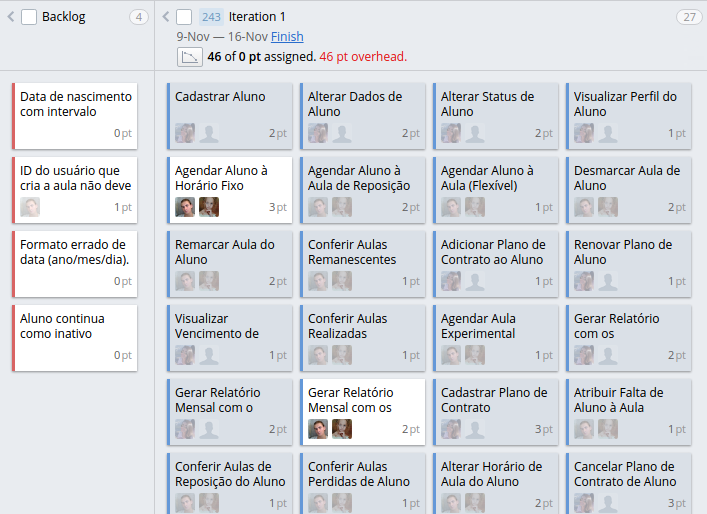
\includegraphics[width=\textwidth]{figuras/plano_iteracao_1.png}
    \caption{Quadro de Plano de Iteração I}
    \label{fig:plano_iteracao_1}
\end{figure}

Estes problemas (ou Bugs) estão ligados à alguma história de usuário em específico, mas não afetam a totalidade de funcionamento da mesma. Com isso, mesmo com problemas conhecidos, as histórias de usuário pouderam ser consideradas como concluídas.





